\chapter{ Resultados}

\section{Fases metodol\'{o}gicas}

\subsection{Visi\'{o}n}
	
	\subsubsection{Enunciado del problema}
	
	El problema que se presenta es que se est\'{a} utilizando el HunterLab Universal Software para el manejo del espectrofot\'{o}metro de reflexi\'{o}n difusa MiniScan XE Plus. Dicho software est\'{a} en ingl\'{e}s, es comercial, privativo y fue descontinuado; esto afecta a los dermat\'{o}logos del CIMBUC.
	
	El impacto causado por esto es que los dermat\'{o}logos encuentran el HunterLab Universal Software dif\'{i}cil de utilizar e imposible de adaptar a sus necesidades, lo que ralentiza la actividad de consulta con sus pacientes, genera la necesidad de disponer de personal especializado para su debido uso y disminuye el potencial de dicho instrumento.
	
	Una soluci\'{o}n satisfactoria ser\'{i}a disponer de un software para el uso del \mbox{MiniScan} XE Plus que est\'{e} en espa\~{n}ol, que sea amigable y mantenible, permitiendo que se adapte a las necesidades de los dermat\'{o}logos.
	
	\subsubsection{Descripci\'{o}n de los usuarios}
	
		\begin{table}[h]
		\small
		\caption[Actores del negocio]{\textit{Actores del negocio} (Fuente: Autor).}
		\centering
		\setlength{\extrarowheight}{\altocelda}
		\begin{tabulary}{\anchotabla}{|c|J|}
			\hline
			\thead{\textbf{\small{Actor}}} & \thead{\textbf{\small{Descripci\'{o}n}}}\\ \hline
			\textbf{Administrador} &
			
			Realiza mediciones.
			
			Consulta las historias m\'{e}dicas de los pacientes y las muestras.
			
			Gestiona los usuarios.
		\\ \hline
			\textbf{Dermat\'{o}logo} &
			
			Realiza mediciones.
			
			Gestiona las historias m\'{e}dicas de los pacientes y las muestras.
			
			Realiza diagn\'{o}sticos a partir de los resultados de las muestras.
		\\ \hline
			\textbf{Investigador} &
			
			Realiza mediciones.
			
			Consulta las historias m\'{e}dicas de los pacientes y las muestras.
			
			Realiza an\'{a}lisis sobre los resultados de las mediciones.\\ \hline
		\end{tabulary}
	\end{table}
	
	\begin{table}[h]
		\small
		\caption[Actores del software]{\textit{Actores del software} (Fuente: Autor).}
		\centering
		\setlength{\extrarowheight}{\altocelda}
		\begin{tabulary}{\anchotabla}{|c|J|c|c|}
			\hline
			\thead{\textbf{\small{Actor}}} & \thead{\textbf{\small{Responsabilidad}}} & \thead{\textbf{\small{Experiencia}}} & \thead{\textbf{\small{Uso}}}\\ \hline
			
			\textbf{Administrador} &
			
			Manejar el MiniScan XE Plus.
			
			Crear, consultar, modificar y eliminar usuarios.
			
			Consultar historias m\'{e}dicas de pacientes.
			
			Consultar muestras de pacientes. &
			Alta &
			Alto\\ \hline
			
			\textbf{Dermat\'{o}logo} &
			
			Manejar el MiniScan XE Plus.
			
			Crear, consultar, modificar y eliminar historias m\'{e}dicas de pacientes.
			
			Crear, consultar, modificar y eliminar muestras de pacientes. &
			Baja &
			Alto\\ \hline
			
			\textbf{Investigador} &
			
			Manejar el MiniScan XE Plus.
			
			Consultar historias m\'{e}dicas de pacientes.
			
			Consultar muestras de pacientes. &
			Media &
			Alto\\ \hline
		\end{tabulary}
	\end{table}
	
	\subsubsection{Resumen del producto}
	
	El software desarrollado, denominado a partir de ahora Spectrasoft, es una aplicaci\'{o}n para el uso del MiniScan XE Plus, destinado a la recuperaci\'{o}n de los datos de medici\'{o}n de dicho instrumento, y a la generaci\'{o}n y gesti\'{o}n de resultados relevantes. Dicho software estar\'{a} orientado a las actividades m\'{e}dicas dermatol\'{o}gicas del CIMBUC. La tabla 4.3 resume los beneficios y las caracter\'{i}sticas m\'{a}s importantes que provee el producto.
	
	\begin{table}[h]
		\small
		\caption[Beneficios y caracter\'{i}sticas principales del producto]{\textit{Beneficios y caracter\'{i}sticas principales del producto} (Fuente: Autor).}
		\centering
		\setlength{\extrarowheight}{\altocelda}
		\begin{tabulary}{\anchotabla}{|J|J|}
			\hline
			\thead{\textbf{\small{Beneficio al cliente}}} & \thead{\textbf{\small{Caracter\'{i}stica que lo soporta}}}\\ \hline
			Se puede conectar, calibrar y realizar mediciones con el MiniScan XE Plus. & 
			Comunicaci\'{o}n con el MiniScan XE Plus y acceso a las caracter\'{i}sticas comunmente utilizadas por el mismo.\\ \hline
			Se dispone de informaci\'{o}n relevante para el an\'{a}lisis y diagn\'{o}stico de patolog\'{i}as dermatol\'{o}gicas en la piel de los pacientes. &
			Muestra de los datos espectrales obtenidos de las mediciones, representaci\'{o}n gr\'{a}fica de dichos datos, y c\'{a}lculo de valores adicionales asociados a los mismos.\\ \hline
			Se pueden gestionar los usuarios, las historias m\'{e}dicas y las muestras generadas de las mediciones. &
			Manejo de una base de datos que almacena toda la informaci\'{o}n referente a los usuarios, las historias m\'{e}dicas y las muestras, permitiendo su gesti\'{o}n por medio del Spectrasoft.\\ \hline
			El Spectrasoft se puede utilizar con facilidad. &
			Interfaz gr\'{a}fica de usuario en espa\~{n}ol, que ofrece \'{u}nicamente las funciones necesarias para gestionar la informaci\'{o}n que necesitan los usuarios. \\ \hline
			El Spectrasoft se puede adaptar a las futuras necesidades de sus usuarios. &
			C\'{o}digo abierto del proyecto disponible en su totalidad para realizar cualquier modificaci\'{o}n y/o extensi\'{o}n.\\ \hline
		\end{tabulary}
	\end{table}
	
	\subsubsection{Principales restricciones}
	
	El software se desarrolla utilizando el lenguaje de programaci\'{o}n C++, empleando \'{u}nicamente tecnolog\'{i}as gratuitas, y en la medida de lo posible, de c\'{o}digo abierto. Se ejecuta en sistemas operativos Windows actuales. Por \'{u}ltimo, la comunicaci\'{o}n entre el software y el MiniScan XE Plus se logra por medio de un puerto serial, o a trav\'{e}s de un adaptador USB.
	
\subsection{Pila del producto \textit{(product backlog)}}
	La lista de requerimientos funcionales que necesitan ser realizados a lo largo del desarrollo del Spectrasoft son el producto de una reuni\'{o}n que se tuvo con los dermat\'{o}logos y los investigadores del CIMBUC, al igual que de la observaci\'{o}n directa efectuada a las funciones que el HunterLab Universal Software ofrece para el manejo del MiniScan XE Plus. En la tabla 4.4 se muestran dichos requerimientos.
	
	\begin{table}[h]
		\small
		\caption[Requerimientos funcionales del software]{\textit{Requerimientos funcionales del software} (Fuente: Autor).}
		\centering
		\setlength{\extrarowheight}{\altocelda}
		\begin{tabulary}{\anchotabla}{|c|J|c|}
			\hline
			\thead{\textbf{\small{C\'{o}digo}}} & \thead{\textbf{\small{Requerimiento}}} & \thead{\textbf{\small{Prioridad}}}\\ \hline
			
			\textbf{RF01} & Conectar y desconectar el MiniScan XE Plus. & Esencial\\ \hline
			
			\textbf{RF02} & Calibrar el MiniScan XE Plus. & Esencial\\ \hline
			
			\textbf{RF03} & Recuperar los 31 puntos espectrales de una medici\'{o}n con el MiniScan XE Plus y mostrarlos en su forma num\'{e}rica. & Esencial\\ \hline

			\textbf{RF04} & Graficar una curva de reflectancia difusa a partir de los 31 puntos espectrales recuperados. & Esencial\\ \hline
			\textbf{RF05} & Graficar una curva de absorbancia aparente a partir de los 31 puntos espectrales recuperados. & Esencial\\ \hline
			\textbf{RF06} & Calcular y mostrar las coordenadas de cromaticidad CIE xyz. & Esencial\\ \hline
			
			\textbf{RF07} & Calcular y mostrar las coordenadas del espacio CIELAB. & Esencial\\ \hline

			\textbf{RF08} & Calcular y graficar el coeficiente de absorci\'{o}n de la epidermis. & Esencial\\ \hline

			\textbf{RF09} & Calcular y mostrar el \'{i}ndice de eritema. & Esencial\\ \hline

			\textbf{RF10} & Almacenar la informaci\'{o}n de los usuarios, las historias m\'{e}dicas, las muestras y los resultados de las mediciones en una base de datos. & Esencial\\ \hline			

			\textbf{RF11} & Gestionar la creaci\'{o}n, consulta, modificaci\'{o}n y eliminaci\'{o}n de los usuarios. & Esencial\\ \hline
			
			\textbf{RF12} & Gestionar la creaci\'{o}n, consulta, modificaci\'{o}n y eliminaci\'{o}n de las historias m\'{e}dicas de pacientes. & Esencial\\ \hline
			
			\textbf{RF13} & Gestionar la creaci\'{o}n, consulta, modificaci\'{o}n y eliminaci\'{o}n de las muestras pertenecientes a las historias m\'{e}dicas. & Esencial\\ \hline	
			
			\textbf{RF14} & Exportar los datos de una muestra a un archivo port\'{a}til. & Esencial\\ \hline
		\end{tabulary}
	\end{table}
	
\subsection{Requerimientos no funcionales}
	
	De la misma forma que los requerimientos funcionales, la lista de los requerimientos no funcionales fue definida en la misma reuni\'{o}n con los dermat\'{o}logos y los investigadores, tomando en cuenta las restricciones del entorno en donde se va a ejecutar el Spectrasoft. En la tabla 4.5 se describen estos requerimientos no funcionales.
	
	\begin{table}[h]
		\small
		\caption[Requerimientos no funcionales del software]{\textit{Requerimientos no funcionales del software} (Fuente: Autor).}
		\centering
		\setlength{\extrarowheight}{\altocelda}
		\begin{tabulary}{\anchotabla}{|c|J|c|}
			\hline
			\thead{\textbf{\small{C\'{o}digo}}} & \thead{\textbf{\small{Requerimiento}}} & \thead{\textbf{\small{Prioridad}}}\\ \hline
			\textbf{RNF01} & El software debe ser f\'{a}cil de utilizar, por lo que debe cumplir con el atributo de usabilidad de un software de calidad. & Esencial\\ \hline
			\textbf{RNF02} & El software debe ser capaz de adaptarse a las necesidades de los dermat\'{o}logos, permitiendo la incorporaci\'{o}n de nuevos requerimientos y funcionalidades, raz\'{o}n por la cual debe cumplir con el atributo de mantenibilidad de un software de calidad. & Esencial\\ \hline
			\textbf{RNF03} & El software debe desarrollarse empleando \'{u}nicamente herramientas y tecnolog\'{i}as gratuitas, y en la medida de lo posible, libres. & Esencial\\ \hline
			\textbf{RNF04} & El software debe ser capaz de ejecutarse en sistemas Windows actuales, con arquitecturas de 32 bits y 64 bits. & Esencial\\ \hline
			\textbf{RNF05} & El software debe conectarse con el MiniScan XE Plus por medio de un puerto serial o de un adaptador USB. & Esencial\\ \hline
			\textbf{RNF06} & El archivo port\'{a}til al que se exportan los resultados de una medici\'{o}n debe ser abierto por un visualizador/editor de hojas de c\'{a}lculo. & Esencial\\ \hline
			\textbf{RNF07} & El software debe desarrollarse utilizando el lenguaje de programaci\'{o}n orientado a objetos C++. & Esencial\\ \hline
		\end{tabulary}
	\end{table}
	
\newpage

\subsection{Casos de uso}

 \begin{itemize}
 	
 	\item \textbf{Operar el MiniScan XE Plus:}
 	
 		\begin{figure}[H]
		\centering
		
\includegraphics[scale=0.4]{img/cu-manejar-miniscan.png}
			\caption[Caso de uso: operar el MiniScan XE Plus]{\textit{Caso de uso: operar el MiniScan XE Plus} (Fuente: Autor).}
	\end{figure}
	
	 	\item \textbf{Gestionar medici\'{o}n:}
 	
 		\begin{figure}[H]
		\centering
		
\includegraphics[scale=0.4]{img/cu-gestion-medicion.png}
			\caption[Caso de uso: gestionar medici\'{o}n]{\textit{Caso de uso: gestionar medici\'{o}n} (Fuente: Autor).}
	\end{figure}

\newpage
	 	\item \textbf{Gestionar sesi\'{o}n de usuario:}
 	
 		\begin{figure}[H]
		\centering
		
\includegraphics[scale=0.5]{img/cu-gestion-sesion.png}
			\caption[Caso de uso: gestionar sesi\'{o}n de usuario]{\textit{Caso de uso: gestionar sesi\'{o}n de usuario} (Fuente: Autor).}
	\end{figure}
	
		 	\item \textbf{Gestionar historia:}
 	
 		\begin{figure}[H]
		\centering
		
\includegraphics[scale=0.5]{img/cu-gestion-historia.png}
			\caption[Caso de uso: gestionar historia]{\textit{Caso de uso: gestionar historia} (Fuente: Autor).}
	\end{figure}

\newpage
		\item \textbf{Gestionar muestra:}
 	
 		\begin{figure}[H]
		\centering
		
\includegraphics[scale=0.5]{img/cu-gestion-muestra.png}
			\caption[Caso de uso: gestionar muestra]{\textit{Caso de uso: gestionar muestra} (Fuente: Autor).}
	\end{figure}
	
		\item \textbf{Gestionar usuario:}
 	
 		\begin{figure}[H]
		\centering
		
\includegraphics[scale=0.5]{img/cu-gestion-usuario2.png}
			\caption[Caso de uso: gestionar usuario]{\textit{Caso de uso: gestionar usuario} (Fuente: Autor).}
		\end{figure}
			
		\item \textbf{Caso de uso general:}
 	
 		\begin{figure}[H]
		\centering
		
\includegraphics[scale=0.6]{img/cu-general.png}
			\caption[Caso de uso general]{\textit{Caso de uso general} (Fuente: Autor).}
		\end{figure}
	
 \end{itemize}
 
\newpage
 
	\subsubsection{Descripci\'{o}n de los casos de uso}
	
		\begin{itemize}
			\item \textbf{Operar MiniScan:} Permite a todos los usuarios conectar, desconectar y calibrar el MiniScan XE Plus, esto \'{u}ltimo haciendo uso de una trampa de luz y una cer\'{a}mica blanca.
			
			\item \textbf{Gestionar medici\'{o}n:} Permite a todos los usuarios efectuar una medici\'{o}n con el MiniScan XE Plus conectado, visualizar los resultados obtenidos de la misma, y borrarlos.
			
			\item \textbf{Consultar medici\'{o}n:} Permite a todos los usuarios visualizar tanto la informaci\'{o}n obtenida directamente del MiniScan XE Plus, como la informaci\'{o}n calculada a partir de la misma, como la curva de reflectancia difusa, la curva de absorbancia aparente, las coordenadas de cromaticidad CIE xyz, las coordenadas CIELAB, el coeficiente de absorci\'{o}n y el \'{i}ndice de eritema de una medici\'{o}n realizada.
			
			\item \textbf{Gestionar sesi\'{o}n de usuario:} Permite a cualquier usuario iniciar sesi\'{o}n para acceder a las funciones pertinentes a su rol, consultar y modificar su informaci\'{o}n, cambiar su contrase\~{n}a, y cerrar sesi\'{o}n.
			
			\item \textbf{Gestionar historia:} Permite a todos los usuarios consultar la informaci\'{o}n perteneciente a las historias m\'{e}dicas, y s\'{o}lo permite a los usuarios con el rol de dermat\'{o}logo registrar, modificar y eliminar dichas historias. 
			
			\item \textbf{Gestionar muestra:} Permite a todos los usuarios consultar la informaci\'{o}n referente a las muestras pertenecientes a una historia m\'{e}dica de un paciente determinado, as\'{i} como exportar dicha informaci\'{o}n, y s\'{o}lo permite a los usuarios con el rol de dermat\'{o}logo registrar, modificar y eliminar tales muestras.
			
			\item \textbf{Gestionar usuario:} Permite registrar usuarios, consultar su informaci\'{o}n, cambiar los roles de dichos usuarios, cambiar sus contrase\~{n}as y eliminarlos. Esto solamente puede ser efectuado por usuarios con el rol de administrador.
		\end{itemize}

\subsection{Glosario}

\begin{itemize}
	
	\item \textbf{Espectroscop\'{i}a de reflectancia difusa:}  t\'{e}cnica con la cual se puede estudiar tejido biol\'{o}gico.

	\item \textbf{Espectrofot\'{o}metro de reflexi\'{o}n difusa:} instrumento de medici\'{o}n del color, que emplea la t\'{e}cnica de espectroscop\'{i}a de reflectancia difusa.
	
	\item \textbf{Medici\'{o}n:} es un proceso b\'{a}sico de la ciencia que consiste en comparar un patr\'{o}n seleccionado con el objeto o fen\'{o}meno cuya magnitud f\'{i}sica se desea medir, para ver cu\'{a}ntas veces el patr\'{o}n est\'{a} contenido en esa magnitud.
	
	\item \textbf{Calibraci\'{o}n:} proceso de comparar los valores obtenidos por un instrumento de medici\'{o}n con la medida correspondiente de un patr\'{o}n de referencia.
	
	\item \textbf{Historia m\'{e}dica:} documento m\'{e}dico-legal que surge del contacto entre el profesional de la salud (en este caso, dermat\'{o}logo) y el paciente, donde se recoge la informaci\'{o}n necesaria para la correcta atenci\'{o}n de los pacientes.
	
	\item \textbf{Muestra:} parte o cantidad peque\~{n}a de una cosa que se considera representativa del total y que se toma o se separa de ella con ciertos m\'{e}todos para someterla a estudio, an\'{a}lisis o experimentaci\'{o}n.
	
	\item \textbf{Patolog\'{i}a dermatol\'{o}gica:} parte de la medicina dermatol\'{o}gica que estudia los trastornos anat\'{o}micos y fisiol\'{o}gicos de la piel, as\'{i} como los s\'{i}ntomas y signos a trav\'{e}s de los cuales se manifiestan las enfermedades y las causas que las producen.
	
	\item \textbf{Datos espectrales:} datos que representan un conjunto de ondas electromagn\'{e}ticas, ordenadas seg\'{u}n su frecuencia.
	
	\item \textbf{Absorbancia aparente:} es la luz que aparentemente est\'{a} siendo absorbida por un medio.
	
	\item \textbf{Coordenadas de cromaticidad CIE xyz:} valores que representan los est\'{i}mulos de la luz de una forma est\'{a}ndar.
	
	\item \textbf{Coordenadas del espacio CIELAB:} valores obtenidos de la transformaci\'{o}n de las coordenadas de cromaticidad CIE xyz, haciendolas representables en un espacio de tres dimensiones.
	
	\item \textbf{Epidermis:} membrana epitelial que recubre la parte m\'{a}s superficial del cuerpo de los animales.	
	
	\item \textbf{Coeficiente de absorci\'{o}n:} conjunto de valores que indican el nivel de concentraci\'{o}n de melanina presente en la epidermis de un paciente.
	
	\item \textbf{\'{I}ndice de eritema:} valor utilizado para determinar el nivel inflamatorio de la epidermis de un paciente.
	
\end{itemize}

\newpage

\section{Base de datos}

	\subsection{Diagrama ER de la base de datos}

	\begin{figure}[H]
		\centering
		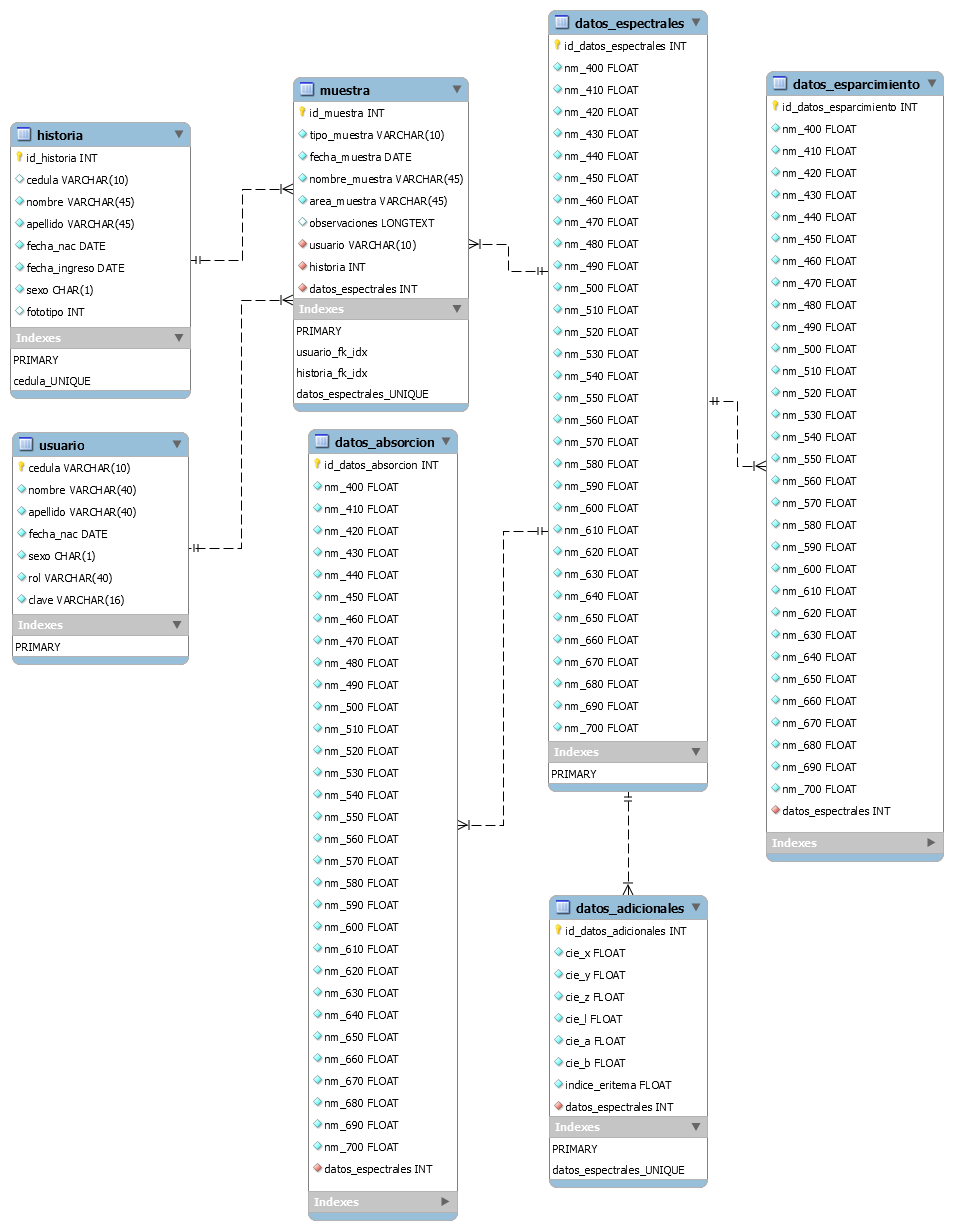
\includegraphics[scale=.4]{img/diagramaER.png}
			\caption[Diagrama ER de la base de datos]{\textit{Diagrama ER de la base de datos} (Fuente: Autor).}
	\end{figure}
	
	\subsection{Descripci\'{o}n de las tablas de la base de datos}
	
		\begin{itemize}
				
				\item \textbf{historia:} almacena los datos referentes a la historia m\'{e}dica de cada uno de los pacientes registrados.
				
				\item \textbf{usuario:} guarda la informaci\'{o}n de cada uno de los usuarios que pueden acceder al software, que pueden ser administradores, dermat\'{o}logos o investigadores.
				
				\item \textbf{muestra:} contiene los datos relevantes de las muestras que son tomadas a los pacientes. Dichas muestras siempre est\'{a}n interrelacionadas con la historia m\'{e}dica del paciente al que pertenece, y la c\'{e}dula del usuario que la tom\'{o}.

				\item \textbf{datos\_espectrales:} contiene los 31 puntos espectrales resultantes de la medici\'{o}n realizada sobre cada muestra por medio del MiniScan XE Plus.
				
				\item \textbf{datos\_absorcion:} contiene los 31 puntos espectrales resultantes del c\'{a}lculo del coeficiente de absorci\'{o}n asociado con los datos espectrales.
				
				\item \textbf{datos\_adicionales:} almacena los datos que son calculados a partir de los 31 puntos espectrales de cada muestra, estos son las coordenadas de cromaticiad CIE xyz, las coordenadas del espacio del color CIELAB y el \'{i}ndice de eritema.
				
		\end{itemize}

\section{Recursos y tecnolog\'{i}as utilizados}

	\subsection{Recursos}
	
		\begin{itemize}
			
			\item \textbf{Adaptador RS232-USB:} es un cable adaptador que habilita la comunicaci\'{o}n de dispositivos que utilizan puerto serial con computadoras que disponen de puertos USB, creando puertos COM virtuales con las mismas mientras se realiza dicha comunicaci\'{o}n. Este cable es utilizado como adaptador para el cable de comunicaci\'{o}n RS232 DB-9 hembra a RJ-45 del MiniScan XE Plus, habilitando su utilizaci\'{o}n en computadoras que no poseen puerto serial.
			
			\item \textbf{MiniScan XE Plus OCX Kit (MSXE.ocx):} es un archivo dise\~{n}ado por la empresa HunterLab para controlar y realizar mediciones con el MiniScan XE Plus. Su objetivo es proporcionar a los desarrolladores un componente reutilizable de software que d\'{e} acceso a las caracter\'{i}sticas comunmente utilizadas por el instrumento.
			
			\item \textbf{MiniScan XE Plus:} es un instrumento de medici\'{o}n del color creado por la empresa HunterLab, de dise\~{n}o compacto y port\'{a}til, que emplea la t\'{e}cnica de espectroscop\'{i}a de reflectancia difusa, el cual se puede apreciar en la figura 4.9. Este instrumento mide la cantidad de luz que refleja una muestra dentro de un rango de longitudes de onda que va desde los 400 hasta los 700 nan\'{o}metros, generando como resultado 31 puntos espectrales dentro de ese rango, que son el insumo principal del Spectrasoft.
			
		\end{itemize}
		
	\begin{figure}[H]
		\centering
		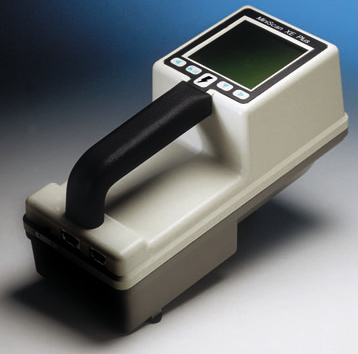
\includegraphics[scale=1]{img/MiniScanXEPlus.png}
			\caption[MiniScan XE Plus]{\textit{MiniScan XE Plus} (Fuente: HunterLab, 2006).}
	\end{figure}

	\subsection{Tecnolog\'{i}as}
	
		\begin{itemize}
			
			\item \textbf{Qt:} es un \textit{framework} de desarrollo de aplicaciones multiplataforma para sistemas operativos de escritorio, sistemas integrados y sistemas m\'{o}viles. Se utiliz\'{o} la versi\'{o}n \textit{open source} 5.4.1 de este \textit{framework} para el desarrollo del Spectrasoft.
			
			\item \textbf{Visual Studio:} es un entorno integrado de desarrollo o \textit{IDE} para crear aplicaciones en varias plataformas, como Windows, Android y iOS. La versi\'{o}n 2013 de este \textit{IDE} fue utilizada para desarrollar una librer\'{i}a escrita en Visual Basic.NET, la cual act\'{u}a como intermediaria entre el kit \textit{MSXE.ocx} y el \textit{framework} Qt, para as\'{i} utilizar las caracter\'{i}sticas del MiniScan XE Plus en el Spectrasoft.
			
			\item \textbf{PostgreSQL:} es un sistema \textit{open source} multiplataforma de bases de datos relacionales. Posee m\'{a}s de 15 a\~{n}os de desarrollo activo y una arquitectura comprobada que se ha ganado una fuerte reputaci\'{o}n por confiabilidad, integridad de datos y correctitud. La versi\'{o}n 9.4.4-3 de este sistema se utiliz\'{o} para desarrollar y administrar la base de datos con la que opera el Spectrasoft.
			
			\item \textbf{Gitlab:} es un servicio de control de versiones que ofrece alojamiento gratuito, tanto p\'{u}blico como privado, de respositorios para proyectos. Se utiliz\'{o} la versi\'{o}n en l\'{i}nea de este servicio para llevar un control de versiones durante el desarrollo del proyecto.
			
			\item \textbf{QCustomPlot:} es un \textit{widget open source} para Qt que permite realizar el trazado y la visualizaci\'{o}n de datos. Este \textit{widget} fue empleado por el Spectrasoft para visualizar la curva de reflectancia difusa y la curva de absorbancia aparente asociadas a los 31 puntos espectrales resultantes de las mediciones.
			
			\item \textbf{QtXlsx:} es una librer\'{i}a \textit{open source} para Qt que permite leer y escribir archivos con extensi\'{o}n xlsx. Esta librer\'{i}a fue utilizada para implementar en el Spectrasoft la opci\'{o}n de exportar los resultados de una muestra a un archivo port\'{a}til, manejable por medio de aplicaciones de hojas de c\'{a}lculo.
		\end{itemize}

\newpage
\section{Comunicaci\'{o}n con el MiniScan XE Plus}

	Para establecer la comunicaci\'{o}n entre el MiniScan XE Plus y el Spectrasoft, se recurri\'{o} a la documentaci\'{o}n del instrumento, en la cual se describe el MSXE.ocx, un archivo que implementa las funciones comunmente utilizadas por dicho instrumento. Se contact\'{o} al personal de soporte t\'{e}cnico de HunterLab por correo electr\'{o}nico, para solicitarle el c\'{o}digo fuente de dicho archivo y la documentaci\'{o}n relativa a su utilizaci\'{o}n que se pudiera proporcionar para la investigaci\'{o}n.
	
	Si bien el personal no comparti\'{o} el c\'{o}digo fuente del archivo, s\'{i} envi\'{o} la documentaci\'{o}n solicitada y un ejemplo de su uso escrito en Visual Basic for Applications (VBA). Primero se intent\'{o} cargar el archivo y utilizarlo directamente en Qt; sin embargo, ocurr\'{i}a un error de compatibilidad de datos al invocar algunas de sus funciones. La soluci\'{o}n a este problema fue desarrollar una librer\'{i}a escrita en Visual Basic .NET, con la cual se pueden invocar todas las funciones de este archivo sin problema alguno.

	As\'{i} pues, por medio del cable adaptador RS232-USB, y empleando la librer\'{i}a escrita en Visual Basic .NET, se logr\'{o} establecer la comunicaci\'{o}n entre el Spectrasoft y el MiniScan XE Plus.
\newpage
\section{F\'{o}rmulas implementadas}
	A continuaci\'{o}n se muestra el c\'{o}digo fuente de las f\'{o}rmulas de \'{o}ptica y colorimetr\'{i}a que fueron definidas en las bases te\'{o}ricas, e implementadas en el Spectrasoft. Dichas f\'{o}rmulas fueron implementadas utilizando el lenguaje de programaci\'{o}n orientada a objetos C++, utilizando punto flotante de presici\'{o}n simple para almacenar los resultados, debido a que el MiniScan XE Plus maneja la misma presici\'{o}n en la realizaci\'{o}n de sus mediciones.
	
	\begin{itemize}
	
	\item \textbf{Funci\'{o}n de \'{i}ndice de eritema:}	
		\begin{lstlisting}
//Calcula el indice de eritema
float eritema(QVector<float> medicion){
    //promRojo: promedio ponderado del color rojo
    float promRojo = (medicion[24]/2.0 + medicion[25]
    + medicion[26] + medicion[27]/2.0)/3.0;

    //promVerde: promedio ponderado del color verde
    float promVerde = (medicion[16]/2.0 + medicion[17]
     + medicion[18]/2.0)/2.0;

    float resultado = 100.0*(log(1.0/promVerde)
     - log(1.0/promRojo));

    return resultado;
}
	\end{lstlisting}
	
\newpage	
	
		\item \textbf{Funci\'{o}n de absorbancia aparente:}
			\begin{lstlisting}
//Calcula los datos de absorbancia aparente
QVector<float> absorbancia(QVector<float> medicion){

	QVector<float> resultado;
	
   	for(int i = 0; i < 31; ++i)
		resultado.push_back(100.0 - medicion[i]);

    return resultado;
}
			\end{lstlisting}
			
		\item \textbf{Funci\'{o}n de coordenadas de cromaticidad CIE xyz:}		
			\begin{lstlisting}
//Calcula las coordenadas de cromaticidad CIE xyz
QVector<float> CIExyz(QVector<float> medicion){
    
    QVector<float> resultado;
    QVector<float> XYZ = CIEXYZ(medicion);
    float x, y, z;

    x = XYZ[0]/(XYZ[0] + XYZ[1] + XYZ[2]);
    y = XYZ[1]/(XYZ[0] + XYZ[1] + XYZ[2]);
    z = XYZ[2]/(XYZ[0] + XYZ[1] + XYZ[2]);

    resultado.push_back(x);
    resultado.push_back(y);
    resultado.push_back(z);

    return resultado;
}
			\end{lstlisting}
			
\newpage
		
		\item \textbf{Funci\'{o}n de valores triest\'{i}mulo CIE XYZ:}
			\begin{lstlisting}
//Calcula los valores triestimulo CIE XYZ
QVector<float> CIEXYZ(QVector<float> medicion){
    
    QVector<float> resultado;
    float auxK, auxX, auxY, auxZ, k, X, Y, Z;

    auxK = auxX = auxY = auxZ = 0.0;

    //realiza las sumatorias indicadas de las formulas
    for(int i = 0; i < 31; ++i){

		auxK+= iluCIED65[i]*yCIE10[i];
        auxX+= medicion[i]*iluCIED65[i]*xCIE10[i];
        auxY+= medicion[i]*iluCIED65[i]*yCIE10[i];
        auxZ+= medicion[i]*iluCIED65[i]*zCIE10[i];
    }

    //calcula la constante k
    k = 100.0/auxK;

    //calcula los valores triestimulo XYZ
    X = k*auxX;
    Y = k*auxY;
    Z = k*auxZ;

    resultado.push_back(X);
    resultado.push_back(Y);
    resultado.push_back(Z);

    return resultado;
}
			\end{lstlisting}

\newpage
		
		\item \textbf{Funci\'{o}n de coordenadas CIELAB:}
			\begin{lstlisting}
//Calcula las coordenadas de del espacio CIELAB
QVector<float> CIELAB(QVector<float> medicion){
    
    QVector<float> resultado;
    QVector<float> XYZ = CIEXYZ(medicion);
    float constante, aux, fXfYfZ[3], L, a, b;

    //calcula la constante utilizada en la formula
    constante = 24.0/116.0;
    constante = pow(constante, 3);

    //calcula las funciones X/Xn, Y/Yn, Z/Zn
    for(int i = 0; i < 3; ++i){

        aux = XYZ[i]/XnYnZn[i];

        if(aux > constante){
            fXfYfZ[i] = pow(aux, 1.0/3.0);
        }else{
            fXfYfZ[i] = (841.0/108.0)*aux + (16.0/116.0);
        }
    }

    //calcula las coordenadas L*a*b*
    L = 116.0*fXfYfZ[1] - 16.0;
    a = 500.0*(fXfYfZ[0] - fXfYfZ[1]);
    b = 200.0*(fXfYfZ[1] - fXfYfZ[2]);

    resultado.push_back(L);
    resultado.push_back(a);
    resultado.push_back(b);

    return resultado;
}
			\end{lstlisting}

\newpage		
		
		\item \textbf{Funci\'{o}n de coeficiente de absorci\'{o}n:}
		
			\begin{lstlisting}
//Calcula el coeficiente de absorcion
QVector<float> absorcion(QVector<float> medicion){

    QVector<float> resultado;
    float rango, aux, Z, k, a0;
    int n, grado;
    bool op = false;//el sistema de ecuaciones a resolver tiene solucion
    
    //son 31 datos, y el grado del polinomio de ajuste es 8
    n = 31; grado = 8;

    double *x = new double[n];
    double *y = new double[n];

    //cargando los datos en x, y
    for(int i = 0; i < n; ++i){
        x[i] = i;
        y[i] = medicion.at(i);
    }

    double **matriz = new double*[grado + 1];

    for (int i = 0; i < grado + 1; ++i)
        matriz[i] = new double[grado + 2];

    //realizando el ajuste polinomial y calculando los coeficientes
    coeficientes(x, y, matriz, grado, n);
    recorrido(matriz, grado + 1, op);

    //a0 esta en la primera fila de la matriz resultante del ajuste
    a0 = matriz[0][grado + 1];
    Z = 0.2796; k = -7.174;
    rango = 400;

    //calculando el coeficiente de absorcion
    for(int i = 0; i < n; ++i){
        aux = Z*exp(k*a0)*6.6*pow(10, 11)*pow(rango, -3.3);
        resultado.push_back(aux);
        rango+=10;
    }

    //liberando la memoria dinamica asiganada
    delete x;
    delete y;

    for(int i = 0; i < grado + 1; ++i)
        delete matriz[i];

    delete matriz;

    return resultado;
}
			\end{lstlisting}

	\end{itemize}

\newpage

\section{Interfaz del software}

	A continuaci\'{o}n se muestran algunas de las ventanas de la interfaz gr\'{a}fica de usuario del Spectrasoft, que comprenden la ventana principal, la ventana de inicio de sesi\'{o}n, la visualizaci\'{o}n de algunos de los resultados de una medici\'{o}n realizada, y los detalles de la historia m\'{e}dica de un paciente.

 \begin{itemize}
 	
 	\item \textbf{Ventana principal:}
 	
 		\begin{figure}[H]
		\centering
		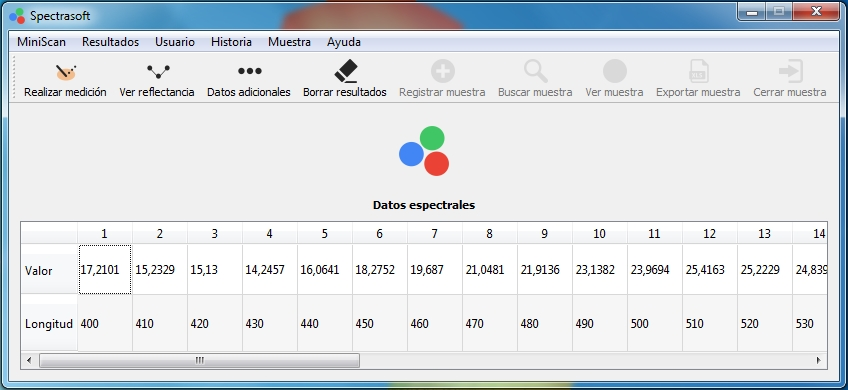
\includegraphics[scale=0.6]{img/vista-principal.jpg}
			\caption[Ventana principal]{\textit{Ventana principal} (Fuente: Autor).}
	\end{figure}
	
	 	\item \textbf{Inicio de sesi\'{o}n:}
 	
 		\begin{figure}[H]
		\centering
		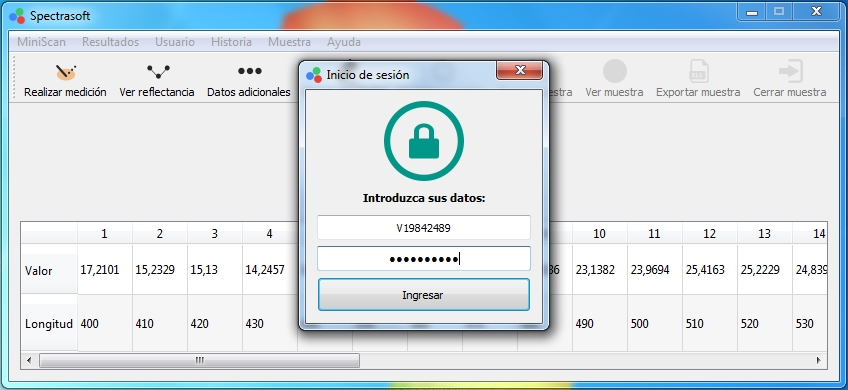
\includegraphics[scale=0.6]{img/vista-inicio-sesion.jpg}
			\caption[Inicio de sesi\'{o}n]{\textit{Inicio de sesi\'{o}n} (Fuente: Autor).}
	\end{figure}

\newpage
	 	\item \textbf{Curva de reflectancia:}
 	
 		\begin{figure}[H]
		\centering
		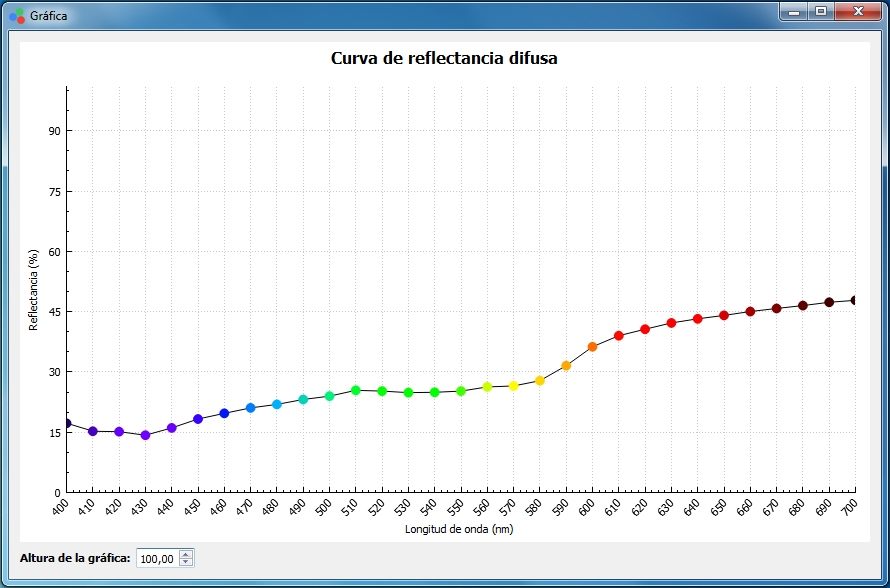
\includegraphics[scale=0.55]{img/vista-reflectancia.jpg}
			\caption[Curva de reflectancia]{\textit{Curva de reflectancia} (Fuente: Autor).}
	\end{figure}
	
		 	\item \textbf{Historia m\'{e}dica de un paciente:}
 	
 		\begin{figure}[H]
		\centering
		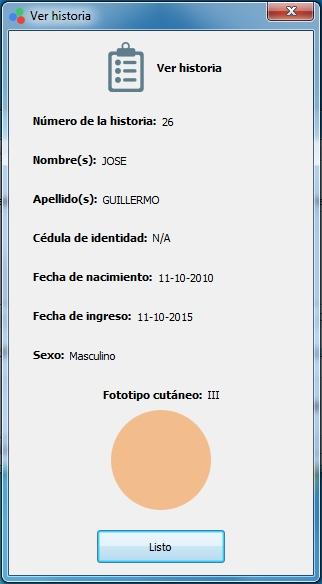
\includegraphics[scale=0.65]{img/vista-historia.jpg}
			\caption[Historia m\'{e}dica de un paciente]{\textit{Historia m\'{e}dica de un paciente} (Fuente: Autor).}
	\end{figure}

\end{itemize}

\newpage
\section{Manuales}
	Se gener\'{o} un manual de instalaci\'{o}n que detalla todos los pasos que se deben seguir para instalar y configurar todo lo necesario para instalar y ejecutar el Spectrasoft, as\'{i} como la instalaci\'{o}n del mismo. Adem\'{a}s se realiz\'{o} un manual de usuario, en donde se explica con detalle la permisolog\'{i}a de los usuarios del Spectrasoft y las funciones que dicho software ofrece. Por \'{u}ltimo, se hizo un manual para el desarrollador, el cual especifica lo que se necesita para desarrollar en el Spectrasoft, y se describen los archivos de c\'{o}digo fuente que conforman dicho proyecto. Estos manuales est\'{a}n disponibles en los anexos A, B y C, respectivamente.

\section{Pruebas realizadas}
	
	El desarrollo de un software incluye verificar y validar que \'{e}ste se encuentre libre de errores y que se haya logrado el objetivo de su dise\~{n}o. En este sentido, se realizaron pruebas de funcionalidad empleando el modelo de guiones de prueba y de pruebas de aceptaci\'{o}n propuestos por \citeA{INSITE}, cuyos resultados permitieron determinar que el software Spectrasoft cumple con todos los requerimientos y objetivos definidos.
	
	Las pruebas de usabilidad se realizaron utilizando las heur\'{i}sticas de \citeA{Nielsen}, tomando \'{u}nicamente los \'{i}tems de evaluaci\'{o}n que se pudieran aplicar en el software y adapt\'{a}ndolos para ese fin. Dichas pruebas de usabilidad mostraron que el software Spectrasoft cumple con el atributo de usabilidad, necesario para ser considerado un software de calidad. Tales pruebas y las constancias de aceptaci\'{o}n firmadas por los clientes est\'{a}n disponibles en los anexos comprendidos desde el D, hasta el G.
	
	\subsection{C\'{a}lculo de los valores triest\'{i}mulo CIE XYZ}
	Para verificar que la implementaci\'{o}n de la f\'{o}rmula para calcular los valores triest\'{i}mulo CIE XYZ	es correcta, se realiz\'{o} una medici\'{o}n a la placa de diagn\'{o}stico de HunterLab con el MiniScan XE Plus, utilizando el Spectrasoft para calcular los valores triest\'{i}mulo de la misma. Esta placa proporciona valores triest\'{i}mulo de control, los cuales fueron le\'{i}dos de f\'{a}brica utilizando el iluminante est\'{a}ndar D65 y el observador est\'{a}ndar de 10 grados. Al comparar los valores triest\'{i}mulo calculados por el Spectrasoft con los valores triest\'{i}mulo de control de la placa, se puede observar que los valores se asemejan. La tabla 4.6 muestra los valores comparados.
	
	\begin{table}[h]
		\small
		\caption[Verificaci\'{o}n de los valores triest\'{i}mulo CIE XYZ]{\textit{Verificaci\'{o}n de los valores triest\'{i}mulo CIE XYZ} (Fuente: Autor).}
		\centering
		\setlength{\extrarowheight}{\altocelda}
		\begin{tabulary}{\anchotabla}{|c|c|}
			\hline
			\thead{\textbf{\small{Valores de control}}} & \thead{\textbf{\small{Valores del Spectrasoft}}}\\ \hline
			$X = 18.6$ & $X = 17.72$\\ \hline
			$Y = 24.5$ & $Y = 23.51$\\ \hline
			$Z = 20.7$ & $Z = 20.01$\\ \hline
		\end{tabulary}
	\end{table}
	
	\subsection{Realizaci\'{o}n de las mediciones}
		Para corroborar que las mediciones realizadas utilizando con el Spectrasoft generan los mismos resultados que las mediciones realizadas con el HunterLab Universal Software, se realiz\'{o} la medici\'{o}n de una muestra en una misma zona dos veces, la primera utilizando el Spectrasoft, y la segunda utilizando el HunterLab Universal Software. En las figuras 4.14 y 4.15 se puede observar que las curvas de reflectancia difusa resultantes de las mediciones tienen la misma forma, por lo que las mediciones realizadas con el Spectrasoft son correctas.
	\newpage
		
 	\begin{figure}[H]
		\centering
		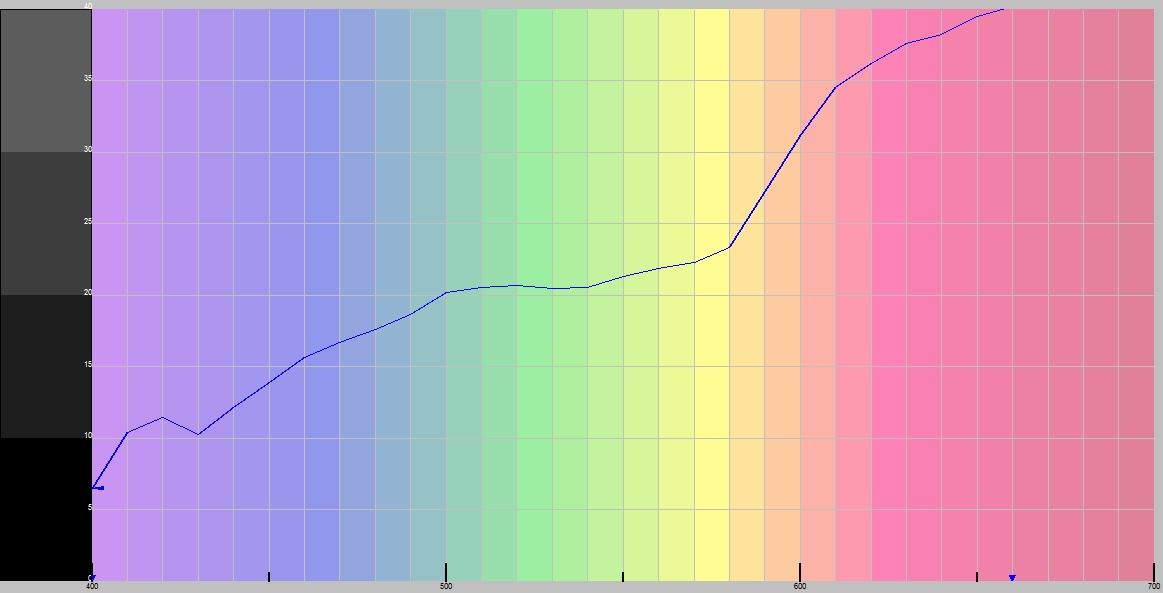
\includegraphics[scale=0.45]{img/medicion-hunterlab.jpg}
			\caption[Medici\'{o}n del HunterLab Universal Software]{\textit{Medici\'{o}n del HunterLab Universal Software} (Fuente: CIMBUC, 2015).}
	\end{figure}	
	
 	\begin{figure}[H]
		\centering
		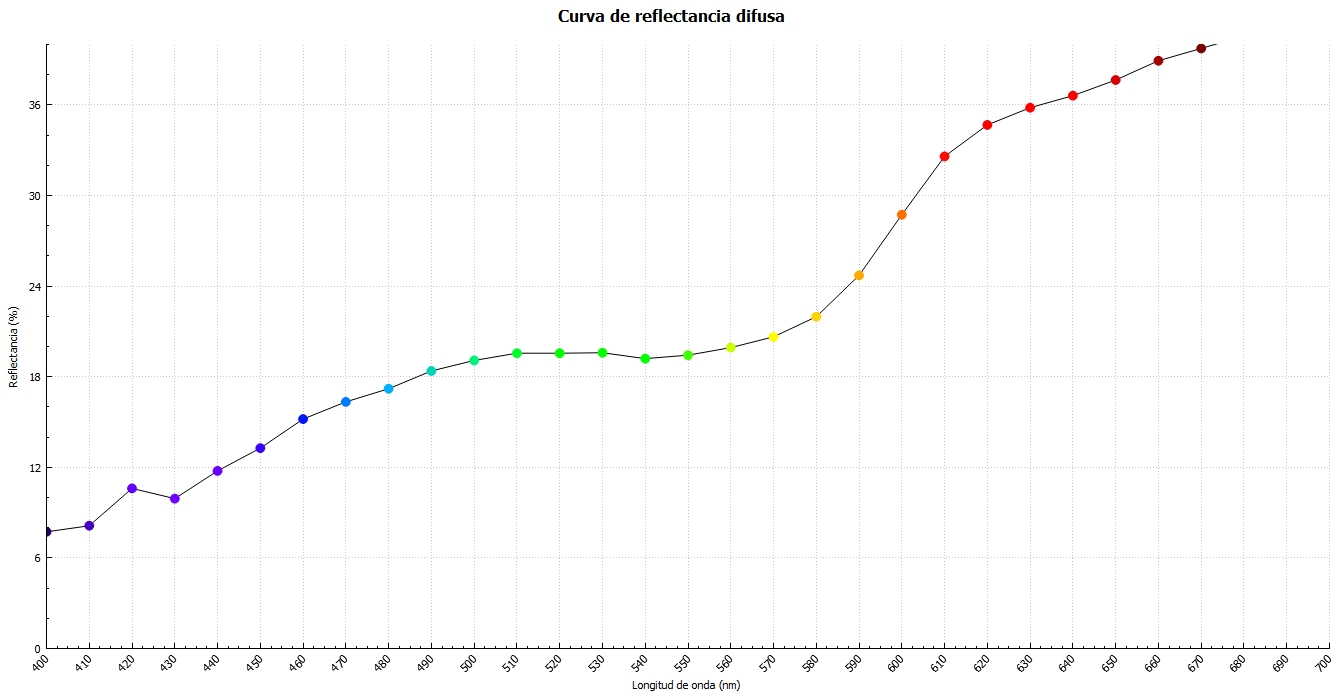
\includegraphics[scale=0.4]{img/medicion-spectrasoft.jpg}
			\caption[Medici\'{o}n del Spectrasoft]{\textit{Medici\'{o}n del Spectrasoft} (Fuente: Autor).}
	\end{figure}
	
\subsection{C\'{a}lculo de las f\'{o}rmulas restantes}

	\begin{itemize}
		
		\item \textbf{Absorbancia aparente:} No hay forma de determinar con exactitud la luz que es absorbida por un medio, por esta raz\'{o}n se asume que la luz que no es reflejada de vuelta al MiniScan XE Plus, debe ser la luz que es aparentemente absorbida. Por esta raz\'{o}n esta f\'{o}rmula no es verificada.
	
		\item \textbf{Coordenadas tricrom\'{a}ticas CIE xyz:} La f\'{o}rmula utilizada para calcular estas coordenadas es una normalizaci\'{o}n de los valores triest\'{i}mulo CIE XYZ, y estos \'{u}ltimos ya fueron verificados, por lo que no hace falta realizar la verificaci\'{o}n de estas coordenadas.
		
		\item \textbf{Coordenadas del espacio CIELAB:} La f\'{o}rmula utilizada para calcular estas coordenadas no es m\'{a}s que la transformaci\'{o}n de los valores triest\'{i}mulo CIE XYZ, raz\'{o}n por la cual no hace falta realizar su verificaci\'{o}n.
		
		\item \textbf{Coeficiente de absorci\'{o}n:} La f\'{o}rmula utilizada para determinar este coeficiente es la definida por \citeA{Narea}, en cuyo art\'{i}culo deja documentadas las pruebas y los an\'{a}lisis relacionados con la misma, por este motivo esta f\'{o}rmula no es verificada.
		
		\item \textbf{\'{I}ndice de eritema:} La f\'{o}rmula utilizada para determinar este \'{i}ndice es la definida por \citeA{Wagner}, en cuyo art\'{i}culo deja documentadas las pruebas y los an\'{a}lisis relacionados con la misma, por esta raz\'{o}n no es verificada.
	\end{itemize}
	
\section{Colores utilizados en el software}

	Es importante destacar que los colores utilizados en las gr\'{a}ficas generadas por el Spectrasoft son referencias visuales, por lo tanto no son una reproducci\'{o}n real de los colores que representan. De la misma manera, los colores utilizados para representar los fototipos de piel en el Spectrasoft son solamente referencias visuales de la escala propuesta por \citeA{Fitzpatrick}.